\documentclass[a4paper,11pt]{article}
\usepackage[utf8]{inputenc} % un package
\usepackage[francais]{babel} %active le mode francais
\usepackage[top=2cm , bottom=2cm , left=2cm , right=2cm]{geometry} %propriétés de notre page
\usepackage{amsmath} %liste de symboles et applications mathématiques
\usepackage{color} %Permet d'utiliser la couleur dans nos documents
\usepackage{listings} %Paquet de coloration syntaxique (langages)
\usepackage{hyperref} % Créer des liens et des signets 
\usepackage[babel=true]{csquotes} %permet les quotations (guillemets)
\usepackage{graphicx} %Importation d'image

% Informations du rapport
\title {Rapport \\ Travaux Pratiques Réseaux (Ethernet)}
\author {Quentin Tonneau - Adrien Lardenois}
\date{}
%Propriétés des liens
\hypersetup{
colorlinks=true, %colorise les liens  
urlcolor= blue, %couleur des hyperliens 
linkcolor= blue,%couleur des liens internes 
} 

\begin{document}
	\maketitle %insère l'en-tête du rapport
	\tableofcontents %insère la table des matières ATTENTION : Compiler deux fois en cas de changements
	\newpage % Nouvelle page
	
	
	
	
	
	
	\section{Introduction}
	Après avoir mis en réseau un parc de pc (cf rapport tp \no 1), nous nous intéressons maintenant à la communication entre ces derniers. En s'appuyant sur le cours de réseaux Ethernet et nos connaissances en langage C dans l'environnement Linux, nous allons concevoir une suite d'applications destinées à interagir avec les PC voisins. Une bibliothèque de création et d'envoi de trame, ainsi qu'un sniffer de réseau (affiche l'ensemble des trames circulant au voisinage de notre matériel) nous sont fournis afin de franchir les couches non étudiées en classe (4,5,6 et 7).
	\subsection{Écouter le réseau}
	Avant de communiquer sur un réseau, il nous faut un certain nombre d'informations sur le matériel avec lequel on souhaite ``entrer en discussion'', c'est à dire :
	%liste à puce
	\begin{itemize}
		\item Le nombre de personnes présentes sur le réseau
		\item Leurs adresses
		\item Le protocole de communication
		\item La nature des messages (émetteur, destinataire, type de message)
	\end{itemize}
	Pour cela, nous concevons un programme qui filtre les trames circulant sur le réseau, en ne conservant que les trames de type 9000 dont nous sommes le destinataire, puis affiche le message en question,tout en dressant une liste de toutes les machines (adresses MAC\footnote{Media access control}) présentes sur le réseau. On pourrait associer ce programme à un module de conversation type IRC\footnote{Internet Relay Tchat}, qui n'affiche que les messages personnels ou à destination de l'ensemble des utilisateurs.
	\subsection{Envoyer un message}
	Après avoir pris connaissance du matériel voisin, nous écrivons une fonction d'envois de trame simple, ainsi qu'un algorithme d'envois en boucle d'un ``bonjour'' sur le réseau (broadcast). Le type choisi pour ces échange est toujours 9000, afin de pouvoir être facilement reçu par les autres groupes du projet. Nous construisons la trame nécessaire, et l'envoyons à l'aide des bibliothèques fournies, et du programme write\_eth\_frame.
	\subsection{Accusé la réception d'un message}
	L'unification des deux parties précédentes nous permet de programmer un répondeur automatique, qui en recevant une trame de type 9000 sous la forme ``Bonjour de XX'' répond immédiatement à son émetteur ``Bonjour de XX : bien reçu par Quentin et Adrien'', accusant ainsi la réception du message. Nous ré-implémentons l'analyse de la première partie, ainsi que nos connaissances en matière de traitement de la langue pour détecter les messages qui nous destinés, et nous utilisons la fonction d'envois de trame crée en deuxième partie pour répondre aux messages.
	\section{Structure du projet}
	\subsection{Structure des trames}
	Avant de nous lancer dans l'écriture des algorithmes de ce projet, nous avons dû analyser les bibliothèques fournies, et définir la structure de notre projet. La structure d'une trame est imposée, sous la forme :
	\lstset{language=C}
	\begin{lstlisting}
	struct eth_frame {
	char adr_dest[6];
	char adr_send[6];
	char type[2];
	char data[1500 - 6 - 6 - 2];
	};
	\end{lstlisting}
	On remarque donc que notre trame sera définie par deux adresses (destinataire et émetteur) MAC au format hexadécimal ($ 6$ octets $\to 12$ caractères), d'un type (même encodage), et de données, n'excédant pas $1500-6-6-2=1486$ caractères. Une structure étant allouée de manière contiguë en mémoire, l'accès à l'adresse de l'émetteur pourra se faire sous la forme trame$\to$adr\_send ou bien (char*)trame[6] .
	\subsection{Arborescence du projet}
	Afin de faciliter la compréhension du projet, l'archive fournie est organisée de la sorte :
	\begin{itemize}
	\item Un fichier de compilation (script sh) se trouve à la racine
	\item Les fichiers sources (.c et .h) utiles au projet sont dans un répertoire \textbf{src}
	\item Une fois compilés, les 5 programmes se trouves dans le répertoire \textbf{bin}
	\end{itemize}
		\renewcommand{\labelitemii}{+}
	Liste et description des fichiers :
	\begin{itemize}
	\item \textbf{compilation.sh} : Fichier de Compilation (voir partie suivante)
	\item \textcolor{blue}{src}
		\begin{itemize}
		\item \textbf{envoyer\_trame .c/.h} : Fichier source de l'envois de trame (bonjour)
		\item \textbf{eth\_lib .c/.h} : Bibliothèque d'utilisation du réseau fournie
		\item \textbf{fonctions .c/.h} : Bibliothèque de fonctions communes au trois principaux programmes
		\item \textbf{inet\_str.h} : Structures des trames, nécessaire à la compilation de eth\_lib
		\item \textbf{recevoir\_trame .c/.h} : Programme d'affichage des trames circulant sur le réseau
		\item \textbf{reponse\_auto .c/.h} : Programme de réponse automatique aux messages reçu (accusé de réception)
		\item \textbf{sniff.c} : Programme de sniff du réseau (fourni)
		\item \textbf{write\_eth\_frame.c} : Programme permettant l'envois de la trame donnée en premier paramètre (fourni)
		\end{itemize}
	\item \textcolor{blue}{bin}
		\begin{itemize}
		\item \textbf{envois} : programme d'envois des bonjours
		\item \textbf{recevoir} : programme d'affichage des trames
		\item \textbf{reponse} : programme d'accusé de réception
		\item \textbf{sniff} : programme utilisé pour l'exécution de recevoir et reponse
		\item \textbf{write\_eth\_frame} : programme appelé par envois et reponse
		\end{itemize}
	\end{itemize}
	\subsection{Compilation et mode d'emplois}
		\subsubsection{Définition des variables avant compilation}
		Afin de compiler les différents algorithmes selon nos besoins, quelques variables (DEFINE) sont à préciser au début de chaque fichier source. En voici la liste :
		\begin{itemize}
		\item envoyer\_trame.c
			\begin{itemize}
			\item NOMBRE\_ENVOIS 200 \textit{Nombre de messages à envoyer}
			\item TEMPS\_ATTENTE 0    \textit{Temps entre deux envois (seconde)}
			\item ADRESSE ``e0:cb:4e:2f:fc:98" \textit{Adresse par défaut de la machine}
			\item MESSAGE``Bonjour de Quentin et Adrien" \textit{Message à envoyer}
			\end{itemize}
		\item recevoir\_trame.c
			\begin{itemize}
			\item TEMPS\_AFFICHAGE 50 \textit{Nombre de trame avant affichage de la liste des adresses}
			\end{itemize}
		\item reponse\_auto.c
			\begin{itemize}
			\item ADRESSE ``e0:cb:4e:2f:fc:98" \textit{Adresse par défaut de la machine}
			\end{itemize}
		\end{itemize}
		\subsubsection{Compilation}
		Pour compiler l'ensemble du projet, il suffit d'exécuter le fichier \textbf{compilation.sh}
		
		Si la compilation échoue, ou pour une architecture spécifique, voici les étapes de la compilation :
		\lstset{language=bash}
		\begin{lstlisting}
	#Cree le repertoire des programmes compiles
	mkdir bin
	#Compile la bibliotheque fournie (necessite inet_str.h)
	gcc src/eth_lib.c -c
	#Compile le logiciel d'envois de trame
	gcc src/write_eth_frame.c eth_lib.o -o bin/write_eth_frame
	#Compile le sniffer
	gcc src/sniff.c eth_lib.o -o bin/sniff
	#Compile le programme d'envois
	gcc src/envoyer_trame.c eth_lib.o src/fonctions.c -o bin/envois
	#Compile le programme d'affichage
	gcc src/recevoir_trame.c eth_lib.o src/fonctions.c -o bin/recevoir
	#Compile le programme de reponse auto
	gcc src/reponse_auto.c eth_lib.o src/fonctions.c -o bin/reponse
	#Supprime le fichier de bibliotheque genere
	rm eth_lib.o
		\end{lstlisting}
		\subsubsection{Notes de compilation}
		Les éventuelles erreur dues à la compilation proviennent des bibliothèques et structures fournies par l'enseignant, mais n'impactent aucunement sur le fonctionnement des différents programmes générés. On remarque également que lors de la compilation du sniffer sur des machines en environnement ``Ubuntu 11.04 et ultérieur version 32bits'' provoque des erreurs lors de l'exécution (segmentation fault). Il est donc conseillé en cas d'erreur de compilation de reprendre les exécutables générés dans l'archive du projet, ou de contacter les auteurs des sources.
		\subsection{Manuel d'Instruction}
		\textbf{ATTENTION : L'ensemble des exécutions doivent se faire à l'aide de droits administrateur. L'utilisation du compte root ou d'une session admin (sudo su) est obligatoire !}
		
		
		
		Les programmes d'envois de trame (reponse et envois) prennent en paramètre l'adresse MAC\footnote{Les lettres doivent y figurer en minuscule} de la machine. Par défaut, l'adresse prise sera l'adresse indiquée dans les sources avant compilation (cf partie ci-dessus). Les programme de réception et d'analyse de trame (reponse et recevoir) doivent posséder en entrée la sortie standard de sniff au moyen d'un ``pipe'' ($|$).\\
		Selon les besoins, voici la liste des commandes d'exécution :
		\begin{itemize}
		\item \textbf{bin/sniff $|$ bin/recevoir} : Affichage des trames (9000) qui circulent sur le réseau
		\item \textbf{bin/sniff $|$ bin/reponse ADRESSEMAC} : Affiche les messages qui nous sont destinés et répond automatiquement
		\item \textbf{bin/envois ADRESSEMAC} :		 Envois une série de trame dans un intervalle de temps (cf partie 2)
		\end{itemize}
		\subsection{Exemple de disposition}
		Pour utiliser pleinement les fonctions de ce projet, il faut donc ouvrir et disposer trois terminaux. Voici un exemple obtenu en plaçant l'afficheur en haut de l'écran, et les autres programmes en bas :\\
		\begin{center} 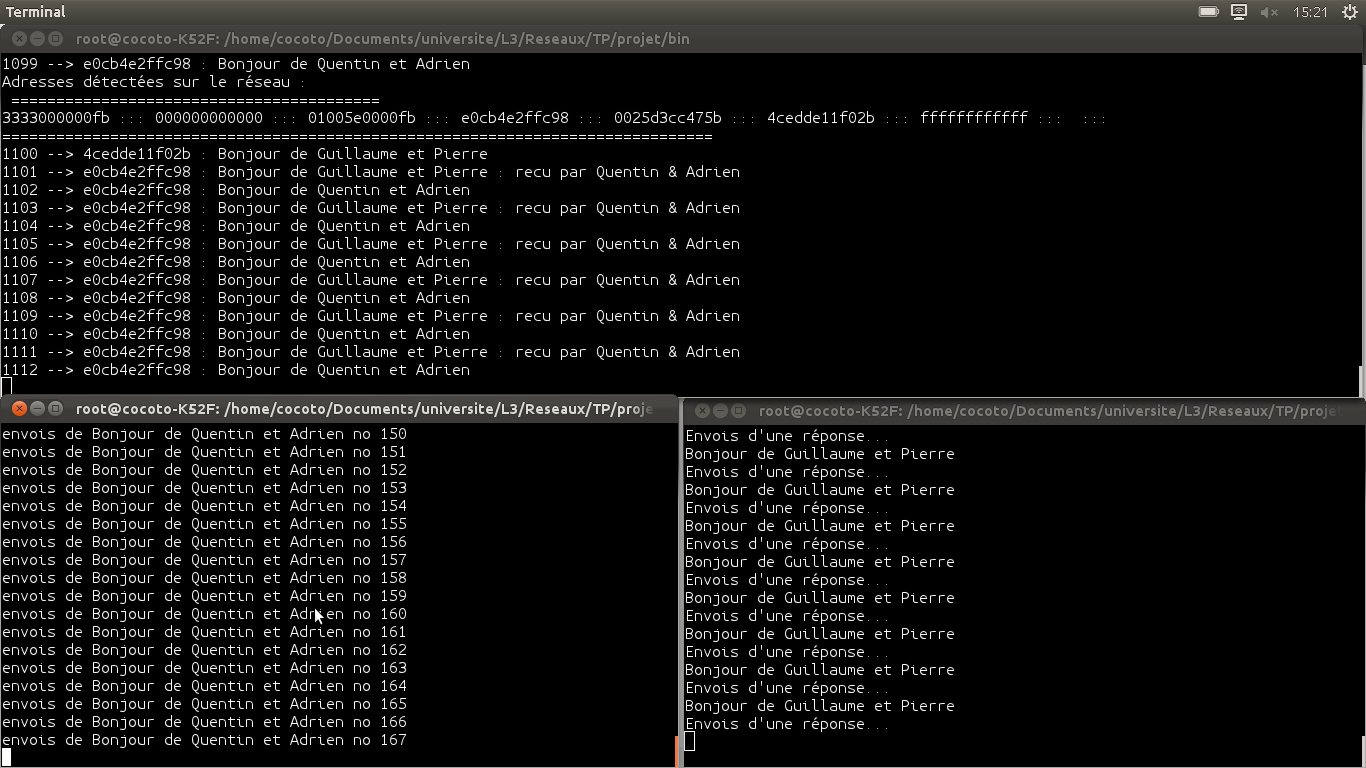
\includegraphics[width=15cm]{capture_ecran_rapport.png}\label{presentation}\end{center}
	\section{Réception des trames}
	La réception de trames se fait par redirection de la sortie du sniffer vers notre programme défini par \textbf{recevoir\_trame.c}, au moyen d'un pipeline.
	Les informations reçues sont traitées une à une par la fonction \textit{lire\_trame()}. On vérifie alors si l'adresse de destination et l'adresse source nous sont déjà connus puis, si l'un et/ou l'autre est ``nouveau'', on l'ajoute à notre liste des matériels connectés.

	Nous avons choisi de représenter la liste des adresses rencontrées par une liste chaînée. Cela a pour avantage de permettre l'ajout d'un maillon sans connaître la taille actuelle de la liste, au contraire d'un tableau qu'il aurai fallu redimensionner au fur et à mesure.
	
	Dans un second temps, on vérifie si la trame appartient au type défini spécialement pour le TP (9000). Si c'est le cas, on affiche à l'écran les informations suivantes :
	\begin{itemize}
		\item Numéro de la trame (au moyen d'un compteur)
		\item Adresse source
		\item Contenu de la trame
	\end{itemize}

	Enfin, chaque fois que Y trames ont été affichées \footnote{Y étant défini au début du programme}, on affiche un récapitulatif des adresses qui circulent sur le réseau. Suivant le choix de Y (50 dans nos exemples) et en fonction du trafic sur le réseau, on bénéficie alors d'un affichage clair des trames qui circulent avec un bilan régulier des utilisateurs présents. %d'ailleurs on pourrai de temps en temps vider la liste pour se débarrasser des utilisateurs inactifs sur le réseau depuis trop longtemps.
	\subsection{la fonction lire\_trame}
	La fonction \textit{lire\_trame} est définie dans \textbf{fonctions.c}. Elle retire les 3 premiers caractères de la sortie du sniffer qui ne nous intéressent pas, puis récupère la longueur de la trame. Après quoi elle capte toute la trame grâce à la fonction \textit{get\_buf} et la retourne en sortie.
	\subsection{la fonction recherche}
	La fonction \textit{ recherche} parcoure la liste chaînée à partir du premier maillon et s'arrête si en passant au suivant elle arrive à NULL. Il est possible de faire le test à la fin car l'initialisation de la liste garanti l'existence d'au moins un maillon différent de NULL.

	Pour chaque maillon, on compare le champ adresse à celle que l'on cherche : s'il y a correspondance on sort directement en renvoyant 1, sinon on passe au suivant. Si la recherche a eu lieu jusqu'au bout sans succès, on retourne 0.
	\subsection{la fonction ajout}
	La fonction d'ajout ajoute un élément en tête de liste. On crée simplement un nouvel élément que l'on défini comme l'adresse à ajouter et dont le suivant est l'ancienne tête de liste.
	\subsection{la fonction affiche}
	La fonction  \textit{affiche} parcoure la liste de la même manière que  \textit{recherche} . Pour chaque étape de la liste, elle affiche l'adresse et sépare les adresses par :::
	\section{Envois des trames (type 9000)}
	\subsection{Fonction d'envois}
	Maintenant que nous recevons les trames de type 9000, nous devons à notre tour envoyer, afin de :
	\begin{itemize}
	\item Nous identifier sur le réseau
	\item Échanger des informations
	\item Accuser la réception d'informations externes
	\end{itemize}
	Pour cela, une fonction nommée ``envois\_trame'' dans le fichier fonctions.c construit la trame en fonctions des paramètres :
	\lstset{language=C}
\begin{lstlisting}
//Envois une trame sur le reseau, de type 9000
void envois_trame(char *source, char *dest, char *message)
\end{lstlisting}
	où source et dest sont les adresses MAC des machines concernées au format XX:XX:XX:XX:XX:XX. Pour cela, nous avons créé une procédure convaddr qui converti les adresses en ajoutant le caractère \enquote{:}. Ensuite, nous créons la trame à l'aide de la fonction
	\lstset{language=C}
\begin{lstlisting}
int make_ping_request(char* eth_addr_dest, char* eth_addr_send,
 char* type_frame, char* data, struct eth_frame* frame);
\end{lstlisting}
	dont la valeur de retour nous indique la taille de la trame générée. Nous convertissons ensuite cette trame au format hexadécimal par la fonction char\_to\_charhexa et nous envoyons la trame en passant cette dernière en paramètre du programme write\_eth\_frame fourni dans le projet.
	\subsection{Programme de présentation}
	Afin de nous présenter une fois connecté sur le réseau, nous avons créé le programme \textit{recevoir\_trame.c} dont les paramètres suivants sont à définir avant la compilation :
	\lstset{language=C}
\begin{lstlisting}
#define NOMBRE_ENVOIS 10  //Nombre de message a envoyer
#define TEMPS_ATTENTE 1	  //Temps d'attente entre deux envois (secondes)
#define ADRESSE "e0:cb:4e:2f:fc:98" //Adresse par defaut
#define MESSAGE "Bonjour de Quentin et Adrien" //Message
\end{lstlisting}
	Ce programme envois un certain nombre de fois un message d'identification sur le réseau, à l'adresse de broadcast \textit{ff:ff:ff:ff:ff:ff}.
	\section{Synthèse et automatisation}
	
	La troisième et dernière partie de notre projet consiste à filtrer les messages qui nous sont adressés et à y répondre par un accusé de réception. Cela est fait par \textbf{reponse\_auto.c}. Par defaut, on défini l'adresse de notre poste mais il est possible de la passer en argument.
	\subsection{fonctionnement global}
	En premier lieu, on vérifie si l'adresse est passée en paramètre, sinon on défini l'adresse à partir de l'adresse par defaut. 
	Puis on commence à écouter les trames.

	Quand on reçoit une trame, on vérifie si elle est de type 9000, si oui : 
	\begin{itemize}
	\item On converti les adresses source et de destination. (car les octets ne sont pas séparés par des ":" à la réception.)
	\item On vérifie : 
		\begin{itemize}
		\item si l'adresse de destination est la notre, ou celle de broadcast
		\item si l'on est pas l'émetteur, afin d'ignorer un de nos messages qui serait broadcasté
		\end{itemize}
	\item Si oui :
		\begin{itemize}
		\item on vérifie que le message n'est pas déjà une reponse (présence d'un ":")
		\item Si ce n'est pas déjà une réponse, on renvoie la trame vers la source en concaténant "reçu par Quentin et Adrien" à la fin de la trame.
	\end{itemize}
	\item Sinon on passe à la suivante
	\end{itemize}

	\subsection{fonctionnement de est\_dans}
	On parcours la chaîne et on retourne 1 dès que l'on trouve le caractère cherché. Si on ne trouve pas on renvoie 0.
	
	\section{Bilan}
	\subsection{Jeux de test et exemples d'utilisation}
	L'ensemble des tests ci-dessous ont étés réalisés en collaboration avec le groupe Pierre Roquin et Guillaume Coutable, sur des ordinateurs personnels reliés par une connexion WIFI ad-hoc.
	\subsubsection{Envois de trame}
	Le fichier \textbf{autres/envois.txt} décrit les sorties console après un échange dans le sens \\PC\_QUENTIN\_ADRIEN $\to$ PC\_PIERRE\_GUILLAUME.
	
	La première partie montre la sortie du programme ``recevoir'', on y retrouve donc nos trames envoyées, ainsi que les réponses du pc distant.
	Arrivé à la trame \no 50, le programme affiche la liste des adresses présentes sur le réseau, conformément aux variables de compilation :
	\begin{lstlisting}
========================================= 
00114304cb38 ::: ffffffffffff ::: 01005e000016 
::: 333300000016 ::: 333300000002 ::: 01005e0000fb ::: 
00266c8a6869 ::: e0cb4e2ffc98 ::: 3333000000fb ::: 000000000000 :::  ::: 
==========================================
	\end{lstlisting}
	On remarque la présence de nos deux adresses MAC respectives (e0cb4e2ffc98 et 00114304cb38), des adresses de broadcast et réseau, ainsi qu'une série d'adresse ``parasites'', que l'on justifie par la présence du réseau WIFI (autres pc souhaitant se connecter, protocoles divers).
	
	La seconde partie nous montre la sortie du programme envoyer.
	
	La troisième partie nous montre la sortie du programme reponse, dans lequel on peut observer uniquement les trames de réponse du PC distant.
	
	\subsubsection{Réception de trame}
	Le fichier \textbf{autres/reception.txt} décrit les sorties console après un échange dans le sens \\PC\_PIERRE\_GUILLAUME $\to$ PC\_QUENTIN\_ADRIEN.
	
	La première partie montre la sortie du programme ``recevoir'', on y retrouve cette fois-ci les messages envoyés par l'autre PC, et nos réponses. Les remarques complémentaires sont identiques à la section ci-dessus
	
	La seconde partie nous montre la sortie du programme reponse, dans lequel on voit les trames envoyées par le PC distant, et un message indiquant que le répondeur a envoyé une trame de réponse automatiquement.
	\subsubsection{Multi-échanges}
	Le fichier \textbf{autres/multi\_echange.txt} décrit les sorties console après un échange dans les deux sens. Les parties sont similaires aux deux premières sections. On remarque lors de l'exécution que l'affichage apparaît subitement après une trentaine de trame.
	
	\subsection{Conclusion}
	L'ensemble du projet nous permet donc de lire les trames circulant sur le réseau, répondre aux trames qui nous sont destinées, et de nous présenter aux autres machines. L'ensemble des exécutables sont utilisables sous environnement UNIX, en Wifi ou Ethernet, selon la définition des variables avant compilation.
	
	Ce projet nous à permis d'exploiter les notions de réseau et trames Ethernet étudiées en cour, d'utiliser le support mis en place lors du tp précédant (mise en réseau des ordinateurs de la salle). De nombreuses versions de code et structure nous ont permis d'exploiter de façon optimale les chaînes de caractères en C, ainsi que l'utilisation des structures et listes-chaînées.
	
	Nous avons rencontré des problèmes lors de la lecture de la bibliothèque fournie, car les fonctions ne sont pas toutes décrites de façon explicite, et les erreurs à la compilation nous ont amené à revoir de nombreuses fois notre code sans comprendre leurs origines. Nous avons également essayé d'utiliser l'interception de signal (exemple Ctrl+C) afin d'afficher la liste des adresses MAC du réseau lors de la fin d'exécution. Mais devant l'instabilité de la solution, nous avons décidé d'abandonner cette option.
	
	Comme indiqué en première partie de ce rapport, l'assemblage des trois exécutables et la présentation proposée en \ref{presentation} nous rappel les solutions de communication de type tchat (Exemple IRC), où chacun peut envoyer un message à destination de tous les utilisateurs, ou bien de ne répondre qu'à la personne choisie. Il aurait été intéressant dans le cadre de ce projet de ré exploiter les fonctions créées afin d'écrire un programme similaire, avec des trames de type 9000, et même un encodage de nos message par divers techniques (RSA).Par exemple, un envois de trame sous le type XXX permet de nous identifier sur le réseau, et les trames de type 9000 concernent les échanges à proprement parlé. Une lecture plus approfondie du sniffer nous aurait également permis d'inclure ses fonctionnalités sous la forme de fonction, et ainsi rendre l'exécution plus simple.
\end{document}
